\chapter{Theoretical Background}

This chapter introduces the concepts used throughout the thesis. It does not attempt to cover all of artificial intelligence, machine learning, or vehicle dynamics. Instead, it builds the vocabulary needed to understand the proposed Trackmania agent: agent, environment, observation, policy, reward, neural network, supervised and imitation learning, reinforcement learning, genetic algorithms, multi-objective evaluation, and geometric virtual sensors.

\section{Artificial Intelligence and Autonomous Decision-Making}

Artificial intelligence can be described broadly as the study of systems that perform tasks requiring intelligence when performed by humans. Turing's classical question of whether machines can exhibit intelligent behavior remains a useful philosophical starting point \cite{turing1950computing}. In a more operational view, Russell and Norvig describe intelligent systems through the idea of agents that perceive their environment and act in it \cite{russell_norvig_aima2021}. This view is especially useful for this thesis, because a racing car in a game can naturally be treated as an agent repeatedly choosing actions.

\paragraph{Control as sequential decision-making.}
Driving is not a one-shot prediction problem. A steering decision changes the future state of the car, which then changes the next decision. This makes racing a sequential decision-making task: the quality of an action is often visible only several steps later. Entering a corner too fast may still look acceptable at the beginning, but it can make the rest of the corner impossible to finish cleanly.

\paragraph{Rule-based and learning systems.}
One way to build behavior is to write rules manually. This is useful when the environment is simple and the desired behavior is well understood. A different way is to let the system learn behavior from data, from interaction, or from optimization. This thesis uses the second direction: the final driving policy is not manually written as a set of rules, but represented by a neural network whose parameters are searched experimentally.

\section{Agent, Environment, and Behavior Policy}

In the terminology used in this thesis, the agent is the decision-making part of the system, while the environment is the world in which its actions have consequences. In our case, the environment is the running Trackmania game together with the reconstructed virtual representation used by the Python runtime.

\paragraph{State, observation, and action.}
The environment has a state, but the agent usually does not receive the complete state directly. Instead, it receives an observation. The observation contains the information selected by the designer as useful for decision-making. The action is the output of the agent that changes the environment. In this thesis, the observation is a compact vector derived from car state and track geometry, and the action is translated into throttle, brake, and steering.

\paragraph{Episode and trajectory.}
A single attempt on a track is treated as an episode. During the episode, the agent produces a sequence of observations and actions. The resulting path of states is a trajectory. This distinction matters because a racing agent is not evaluated by one isolated decision, but by the whole drive.

\paragraph{Behavior policy.}
The behavior policy, usually denoted by \(\pi\), maps observations to actions:
\[
    a_t = \pi(o_t).
\]
Here \(o_t\) is the observation at time \(t\) and \(a_t\) is the action chosen by the agent. Later chapters represent \(\pi\) by a neural network.

\paragraph{Action space.}
The action space describes which actions the agent can choose. It can be discrete, for example a small set of key presses, or continuous, for example an analog steering value. Continuous steering is important for racing because small corrections can matter at high speed.

\paragraph{Type of environment and timing.}
For this thesis, two distinctions are important. A deterministic environment reacts the same way to the same state and action, while a stochastic environment includes randomness or variability. A synchronous environment advances only when the agent requests the next step, while a real-time environment continues running even if the agent is late. Trackmania is practically a real-time environment, and timing variability can make evaluation less ideal than in a fully controlled simulator.

\paragraph{Closed control loop.}
The agent repeatedly receives an observation, selects an action, applies it, and observes the next state. This loop is shown in Figure~\ref{fig:agent-environment-loop}.

\begin{figure}[!htbp]
    \centering
    
\includegraphics[width=\textwidth]{theory/theory_agent_environment_loop.pdf}
    \caption[Agent interaction with the environment]{Basic interaction between an agent and its environment. Sensors provide the agent with an observation and reward, the behavior policy selects an action, and actuators transfer it back to the environment. In the environment, the action causes a transition from state \(s_t\) to the next state \(s_{t+1}\). The scheme follows the general agent--environment model of Russell and Norvig \cite{russell_norvig_aima2021}.}
    \label{fig:agent-environment-loop}
\end{figure}

\section{Evaluating Agent Behavior}

An autonomous agent needs not only a policy, but also a way to evaluate whether one behavior is better than another. In racing, the most obvious metric is time, but time alone is not enough: a very fast crash is not better than a slower clean finish.

\paragraph{Reward and return.}
In reinforcement learning, a reward is a scalar signal obtained after an action, and the return is the accumulated reward over time \cite{sutton_barto2018rl}. In a racing task, reward may be related to progress, speed, finishing, or penalties for crashes.

\paragraph{Optimization objective.}
The objective defines what the training algorithm should improve. If the objective is poorly designed, the agent can learn behavior that maximizes the number but is not actually desirable. This is one reason why the design of the evaluation function becomes a central part of the thesis.

\paragraph{Reward, fitness, and loss.}
Different learning methods use different names for evaluation. Supervised learning minimizes a loss function, reinforcement learning maximizes return, and genetic algorithms maximize fitness. In all cases, however, the designer chooses a signal that tells the algorithm what should count as improvement.

\paragraph{One number and multiple goals.}
Driving contains several goals at once: finish the track, make progress, minimize time, and avoid crashes. A common approach is to combine them into one scalar value with weights. This can work, but the weights are often hard to interpret.

\paragraph{Lexicographic comparison.}
An alternative is to keep criteria separate and compare them in a fixed priority order. For example, a finishing run can be preferred over a non-finishing one before comparing time. Lexicographic ordering is a standard way of handling ordered criteria in multi-criteria optimization \cite{ehrgott2005multicriteria}. Figure~\ref{fig:scalar-vs-lexicographic} shows the difference between scalar and lexicographic evaluation.

\begin{figure}[htbp]
    \centering
    
\includegraphics[width=0.95\textwidth]{theory/theory_scalar_vs_lexicographic.pdf}
    \caption[Scalar and lexicographic evaluation]{Two views of evaluation with multiple metrics. The scalar approach mixes metrics into one number using weights, while lexicographic ordering keeps metrics separate and compares them according to fixed priorities.}
    \label{fig:scalar-vs-lexicographic}
\end{figure}

\paragraph{Risk of poorly designed evaluation.}
Reward shaping can accelerate learning, but it can also change the task if the reward is not aligned with the intended behavior \cite{ng1999shaping}. Reward misdesign is therefore not a small implementation detail; it can become the main reason why an agent learns the wrong thing \cite{knox2023reward_misdesign}.

\section{Neural Networks as Function Approximators}

Neural networks are useful in this thesis because they can represent a policy as a parameterized function. Instead of manually writing a rule for every situation, we search for parameters of a function that maps observations to actions.

\paragraph{Neuron and layer.}
A neuron computes a weighted sum of inputs and applies a nonlinear activation function. A layer contains multiple neurons, and a neural network composes several layers. The basic structure is shown in Figure~\ref{fig:neuron-layer-mlp}.

\begin{figure}[htbp]
    \centering
    
\includegraphics[width=\textwidth]{theory/theory_neuron_layer_mlp.pdf}
    \caption[Neural network]{From a single neuron through a layer to a multilayer feed-forward network. The layers gradually transform the input vector into an output vector, which can represent, for example, an agent action.}
    \label{fig:neuron-layer-mlp}
\end{figure}

\paragraph{Activation functions.}
Activation functions introduce nonlinearity. Without them, multiple linear layers would still form only a linear mapping. Figure~\ref{fig:activation-functions} shows three common choices: sigmoid, hyperbolic tangent, and ReLU.

\begin{figure}[htbp]
    \centering
    
\includegraphics[width=\textwidth]{theory/theory_activation_functions.pdf}
    \caption[Activation functions]{Examples of basic activation functions. Sigmoid restricts the output to \([0,1]\), hyperbolic tangent to \([-1,1]\), and ReLU keeps positive inputs while suppressing negative values to zero.}
    \label{fig:activation-functions}
\end{figure}

\paragraph{Multilayer network and forward pass.}
For a feed-forward network, the output of one layer becomes the input of the next. If \(x\) is the input vector, a layer can be written as
\[
    h = \sigma(Wx+b),
\]
where \(W\) is a matrix of weights, \(b\) is a bias vector, and \(\sigma\) is an activation function. Stacking such layers creates a nonlinear mapping.

\paragraph{Network as a function approximator.}
The universal approximation result by Cybenko shows that feed-forward networks with suitable nonlinear activation can approximate a broad class of functions under certain conditions \cite{cybenko1989approximation}. In practice, this does not say which concrete architecture will work best, but it supports using neural networks as flexible policy representations.

\begin{figure}[htbp]
    \centering
    
\includegraphics[width=0.82\textwidth]{theory/theory_blackbox_function.pdf}
    \caption[Model as function approximation]{Simplified view of a parametric model as a function mapping an input vector to an output vector. From the outside, it can also be seen as a black box whose internal parameters determine the resulting mapping.}
    \label{fig:blackbox-function}
\end{figure}

\paragraph{Network parameters as a search space.}
Once the architecture is fixed, the weights and biases form a vector of parameters. Training means searching this parameter space for values that produce useful behavior. This view connects supervised learning, reinforcement learning, and neuroevolution.

\paragraph{Policy represented by a neural network.}
In this thesis, the policy is represented as
\[
    \pi_\theta(o_t)=a_t,
\]
where \(\theta\) denotes network parameters. The rest of the work investigates how to choose the architecture and how to search for \(\theta\).

\section{Machine Learning Techniques}

This thesis uses several learning concepts, but each plays a different role.

\paragraph{Supervised learning.}
Supervised learning uses input-output pairs. In our case, human driving data provide observations and actions. This is useful for testing whether the observation contains enough information and for selecting a practical network architecture.

\paragraph{Imitation learning.}
Imitation learning tries to reproduce expert behavior. It is natural for driving, but it suffers when the agent enters states not present in the demonstrations. This distribution-shift problem motivates methods such as DAgger \cite{ross2011dagger} and also motivates our later interactive imitation experiment.

\paragraph{Unsupervised learning.}
Unsupervised learning searches for structure without explicit target outputs. It is not a central method in this thesis, but it belongs to the broader family of machine-learning approaches.

\paragraph{Reinforcement learning.}
Reinforcement learning trains an agent through interaction with an environment and a reward signal \cite{sutton_barto2018rl}. It is conceptually well suited for driving, but can require many attempts and careful reward design.

\paragraph{Genetic algorithms.}
Genetic algorithms search over a population of candidate solutions using selection, crossover, mutation, and elitism \cite{goldberg1989ga}. In this thesis, they are used to evolve neural-network parameters.

\paragraph{Common view of policy optimization.}
All these methods can be understood as different ways of searching for a policy: by matching recorded actions, by maximizing reward, or by selecting better individuals in a population.

\section{Reinforcement Learning}

\paragraph{Markov decision process.}
A Markov decision process describes sequential decision-making using states, actions, transition dynamics, rewards, and a discount factor \cite{sutton_barto2018rl}. It is a useful theoretical model, even if the actual Trackmania environment is accessed through a practical runtime interface.

\paragraph{Policy and return.}
The policy selects actions and the return summarizes future rewards. The goal is to find a policy with high expected return.

\paragraph{Value function.}
Value functions estimate how good a state or state-action pair is under a policy. They are central in many reinforcement-learning algorithms \cite{sutton_barto2018rl}.

\paragraph{Exploration and exploitation.}
The agent must explore new behavior while also exploiting behavior that already appears useful. In racing, too little exploration can trap the agent in poor driving, while too much exploration can lead to many crashes.

\paragraph{Sparse reward and reward shaping.}
If the agent receives a strong signal only after finishing the track, learning can be very slow. Reward shaping adds intermediate feedback, but must be designed carefully so that it does not change the intended objective \cite{ng1999shaping}.

\paragraph{Policy-gradient and actor-critic approaches.}
Policy-gradient methods optimize the policy directly, while actor-critic methods combine a policy with a value estimate. These ideas motivate algorithms such as PPO, SAC, and TD3 \cite{sutton_barto2018rl}.

\paragraph{PPO, SAC, and TD3 in this thesis.}
This thesis later uses PPO, SAC, and TD3 only as comparison branches. PPO is a policy-gradient method designed for stable updates \cite{schulman2017ppo}; SAC is an off-policy actor-critic method with entropy regularization \cite{haarnoja2018sac}; TD3 improves deterministic actor-critic learning by reducing overestimation and instability \cite{fujimoto2018td3}. Stable-Baselines3 provides practical implementations of these algorithms \cite{raffin2021sb3}.

\section{Genetic Algorithms and Neuroevolution}

Genetic algorithms are population-based optimization methods inspired by evolution \cite{goldberg1989ga}. They are useful when we can evaluate complete candidate solutions but do not have gradients through the environment.

\paragraph{Population of candidates.}
The algorithm starts with a population of individuals. In this thesis, an individual is a neural network policy represented by its parameters.

\begin{figure}[htbp]
    \centering
    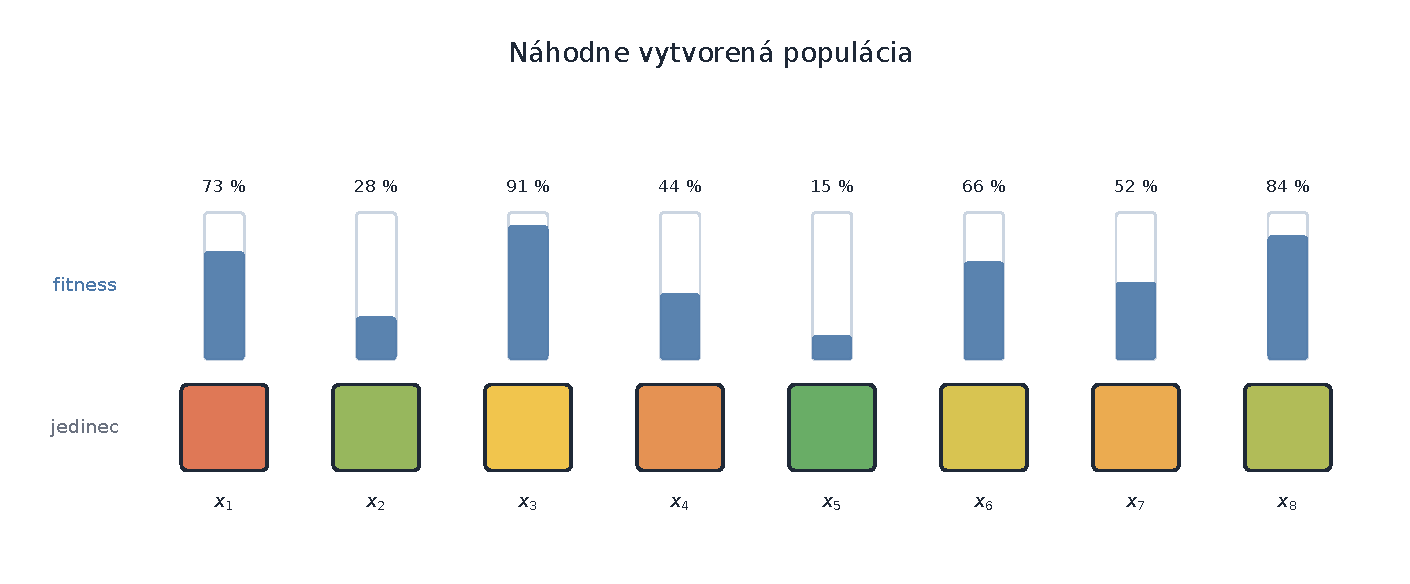
\includegraphics[width=\textwidth]{images/theory/theory_ga_initial_population.pdf}
    \caption[Population initialization]{Initialization of a genetic-algorithm population.}
    \label{fig:ga_initial_population}
\end{figure}

\paragraph{Fitness function.}
Each individual is evaluated by running it in the environment. Its driving behavior produces metrics such as completion, progress, time, and crashes. These metrics are then used to compare individuals.

\paragraph{Parent selection.}
Selection chooses individuals that will produce the next generation. Better individuals are more likely to influence the future population.

\begin{figure}[htbp]
    \centering
    
\includegraphics[width=\textwidth]{images/theory/theory_ga_selection.pdf}
    \caption[Individual selection]{Selection of individuals according to fitness evaluation.}
    \label{fig:ga_selection}
\end{figure}

\paragraph{Crossover.}
Crossover combines information from two parents. For neural-network parameters, this means combining parts of parameter vectors.

\paragraph{Elitism.}
Elitism copies the best individuals directly into the next generation. It protects good solutions from being lost through random variation.

\begin{figure}[htbp]
    \centering
    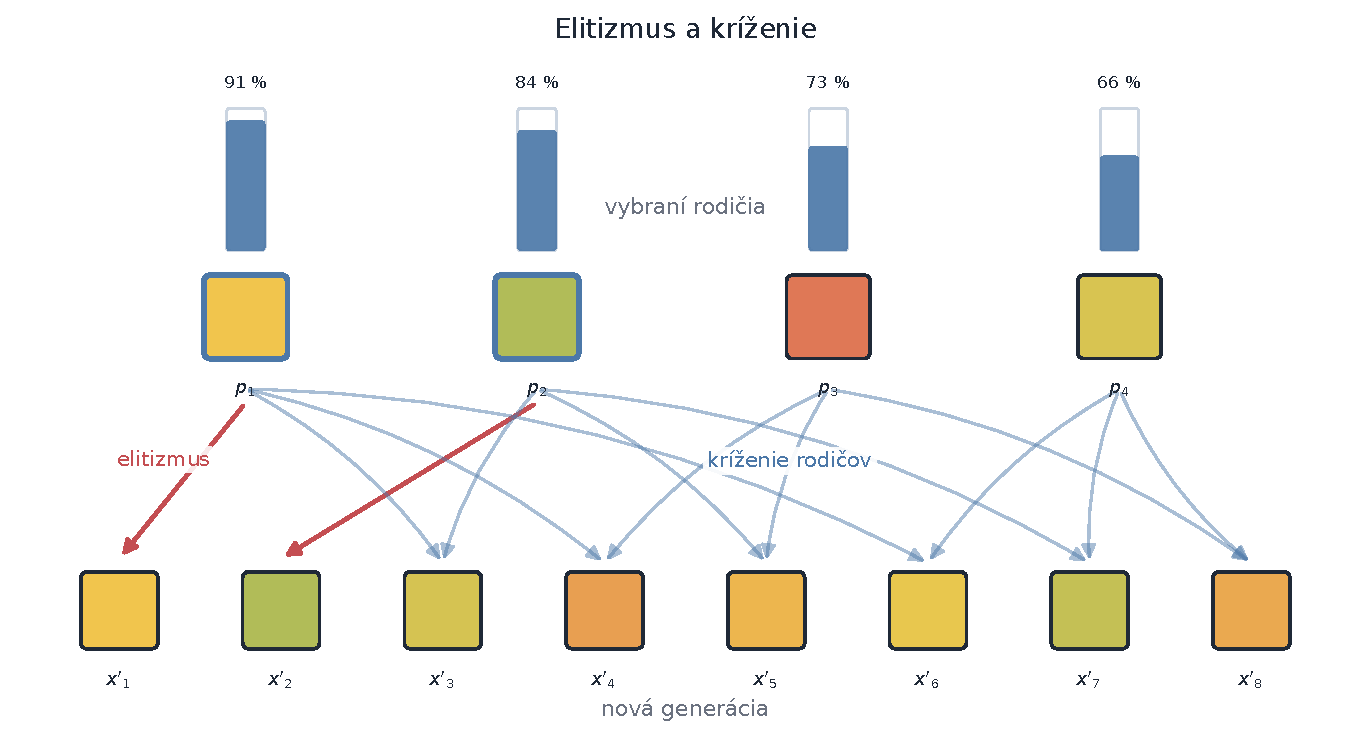
\includegraphics[width=\textwidth]{images/theory/theory_ga_crossover.pdf}
    \caption[Crossover and elitism]{Parent crossover and elitism.}
    \label{fig:ga_crossover}
\end{figure}

\paragraph{Mutation.}
Mutation introduces random changes into offspring. It is the main source of exploration after initialization.

\begin{figure}[htbp]
    \centering
    
\includegraphics[width=0.9\textwidth]{images/theory/theory_ga_mutation.pdf}
    \caption[Offspring mutation]{Mutation of offspring.}
    \label{fig:ga_mutation}
\end{figure}

\paragraph{Exploration and fine-tuning.}
Large mutations help explore the parameter space, while smaller mutations help refine already promising behavior. The balance between these two roles is one of the later experimental questions.

\paragraph{Neuroevolution.}
Neuroevolution applies evolutionary algorithms to neural networks. The genome can represent the network weights, the architecture, or both \cite{stanley2002neat, yao1999_evolving_ann}. In this thesis, the architecture is fixed and the genome represents the parameters.

\begin{figure}[htbp]
    \centering
    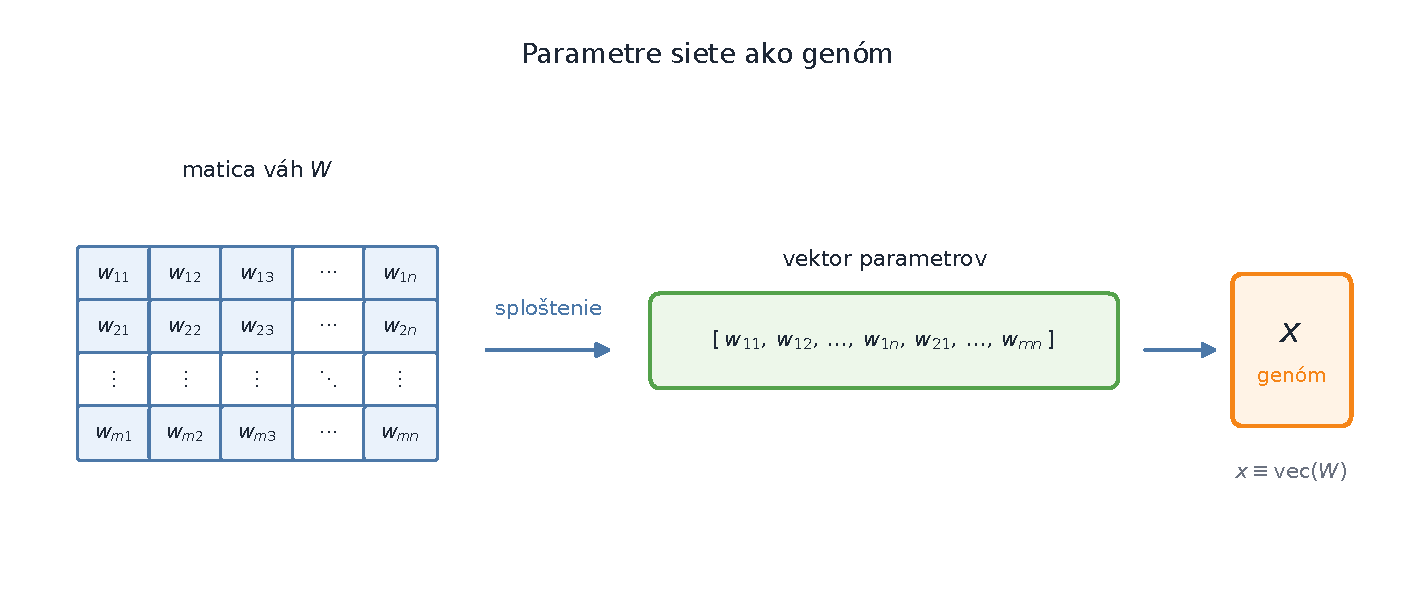
\includegraphics[width=0.92\textwidth]{images/theory/theory_neuroevolution_genome.pdf}
    \caption[Network parameters as genome]{Network parameters as a genome for neuroevolution.}
    \label{fig:neuroevolution_genome}
\end{figure}

\paragraph{Advantages and limitations.}
The advantage of neuroevolution is that it evaluates the whole behavior directly in the environment. The limitation is computational cost: many candidates must be driven and measured.

\section{Multi-Objective Optimization}

Driving contains conflicting objectives. A very safe driver may be slow, while an aggressive driver may be fast but crash often. Multi-objective optimization provides vocabulary for such situations \cite{coello1999survey}.

\paragraph{Conflicting objectives.}
Progress, time, and safety do not always agree. This is why the thesis later compares scalar, lexicographic, and Pareto-based evaluation.

\paragraph{Scalar aggregation.}
Scalar aggregation combines several metrics into one number using weights. It is simple, but the weights may become opaque design constants.

\paragraph{Lexicographic ordering.}
Lexicographic ordering compares metrics by priority. For example, finishing can be more important than time, and time can be more important than the number of minor touches.

\paragraph{Pareto dominance.}
An individual Pareto-dominates another if it is no worse in all objectives and better in at least one. This avoids manually collapsing all objectives into one number.

\paragraph{Pareto front.}
The Pareto front is the set of non-dominated solutions. It shows different trade-offs between objectives.

\paragraph{NSGA-II.}
NSGA-II is a well-known evolutionary multi-objective algorithm that uses non-dominated sorting and diversity preservation \cite{deb2002nsga2}.

\paragraph{Meaning for agent evaluation.}
For this thesis, multi-objective optimization is important because it clarifies why reward design is difficult. It also motivates a later comparison between lexicographic ranking and Pareto-based selection.

\section{Simulations and Virtual Environments}

Virtual environments are useful because they allow repeated experiments without physical risk. OpenAI Gym popularized a simple interface for reinforcement-learning environments \cite{brockman2016openai_gym}, and CARLA is an example of a simulator for autonomous driving research \cite{dosovitskiy2017carla}. Trackmania is not a research simulator, but it offers a precise and repeatable racing environment. The challenge is that it must be connected to an agent through practical runtime tools rather than through a clean research API.

\section{Trackmania as an Environment for an Agent}

\Trackmania{} is a racing game focused on time-attack driving, track building, and repeated improvement of lap time \cite{ubisoft_trackmania2026, trackmania_wiki2026}. Its block-based maps are especially interesting for this thesis because they make geometric reconstruction possible. The game is also suitable for comparison with human driving because performance is measured directly by time.

To illustrate the importance of small time differences, Figure~\ref{fig:trackmania_a01_human_times} shows public leaderboard times for the iconic map \emph{A01-Race}. The figure is not used as a statistical model of all players; it only provides context that tenths of a second can correspond to meaningful differences in ranking.

\begin{figure}[htbp]
    \centering
    
\includegraphics[width=\textwidth]{images/theory/theory_trackmania_a01_human_times.pdf}
    \caption[Human times on A01-Race]{Distribution of the top 1000 times from the public leaderboard of \emph{A01-Race}. The histogram and smoothed curve serve only as a visual representation of the sample; we do not claim that the times are normally distributed. The data were derived from public records for this map \cite{tmnf_exchange_a01_race2026, maniaexchange_api2026}.}
    \label{fig:trackmania_a01_human_times}
\end{figure}

\section{Basic Concepts of Vehicle Control and Racing}

Racing depends on speed, steering, braking, and grip. A car can move forward while also sliding sideways; this lateral motion is important because it can indicate loss of traction. Vehicle dynamics literature describes such relationships through velocity components, slip, and tire-road interaction \cite{rajamani2012vehicle_dynamics}. In this thesis, we do not build a full physical model of the car. We use only selected signals that are useful for the agent observation.

\section{Basics of Computer Graphics for Virtual Sensors}

The proposed agent uses virtual sensors computed over reconstructed geometry. For this, a few computer-graphics concepts are needed.

\paragraph{Geometry of the virtual world.}
The virtual world is represented in a coordinate system. Objects are placed by transformations such as translation and rotation \cite{dunn2011mathprimer}.

\paragraph{Triangle mesh.}
A triangle mesh represents a surface as a set of triangles. This representation is common in computer graphics and is convenient for intersection tests \cite{hughes2014computer_graphics}. Figure~\ref{fig:bunny_mesh_overview} shows a triangle mesh example.

\begin{figure}[htbp]
    \centering
    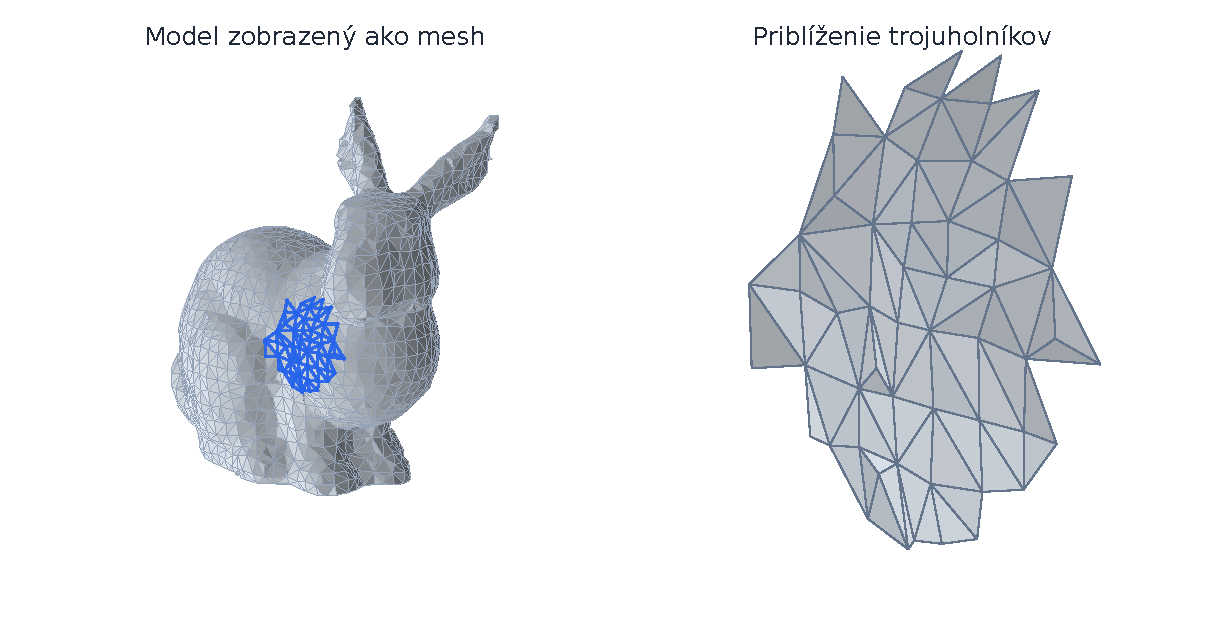
\includegraphics[width=\textwidth]{images/theory/theory_bunny_mesh_overview.pdf}
    \caption[Triangle mesh model]{Triangle mesh of the Stanford Bunny model and a zoomed view of its local structure. The model geometry comes from the Stanford 3D Scanning Repository maintained by the Stanford University Computer Graphics Laboratory \cite{stanford3dscanrep2026}.}
    \label{fig:bunny_mesh_overview}
\end{figure}

\paragraph{Raycasting.}
Raycasting sends a ray into the scene and finds the first intersection with geometry. The Möller--Trumbore algorithm is a standard method for ray-triangle intersection \cite{moller1997raytriangle}. Figure~\ref{fig:mesh_raycasting_detail} illustrates the idea.

\begin{figure}[htbp]
    \centering
    
\includegraphics[width=0.82\textwidth]{images/theory/theory_mesh_raycasting_detail.pdf}
    \caption[Raycasting on a triangle mesh]{Illustration of a ray intersecting a triangle mesh. The highlighting of the ray, direction, and intersection point was created for this thesis; the Stanford Bunny geometry comes from the Stanford 3D Scanning Repository maintained by the Stanford University Computer Graphics Laboratory \cite{stanford3dscanrep2026}.}
    \label{fig:mesh_raycasting_detail}
\end{figure}

\paragraph{Virtual sensors.}
In this thesis, virtual sensors are geometric measurements computed in software. They do not physically exist in the game, but they give the agent information similar to distances, directions, and local track structure. This makes it possible to replace raw image perception with a compact observation vector.
